\section{课题背景}
近年来,随着多核处理器的出现和迅速发展,并行计算、多线程程序逐渐在软件开发领域得到了广泛的使用。与此同时,并行计算的广泛使用也给软件测试提出了新的挑战。
\subsection{程序的并发错误}
因为并行程序本身的特点和缺乏有效的并行程序设计方法与工具,使得正确编写并行程序,调试和优化并行程序都很困难。一方面,编写并行程序比编写串行程序更加困难。除了串行程序常见的错误\footnote{在本篇论文中,漏洞、缺陷、错误可以互换地使用。}之外,并行程序还有诸如死锁、数据争用等独有的错误。所以一段并行程序中存在错误的可能性更大。另一方面,测试并行程序比测试串行程序更加困难。这是因为:第一,并行程序的运行结果具有不确定性,难以重现错误;第二,程序的运行结果牵涉到多线程操作,使得错误不易定位\cite{mcdowell1989debugging}。\par
微软公司在2007年发布的针对684名员工的调查报告显示66\%的受访者需要经常处理并发程序中的问题(包括测试、调试、修复)。超过72\% 的受访者认为重现并行程序中的错误困难或非常困难,63.4\%的受访者需要花费数天才能解决并行程序中的错误。在微软公司的调查报告中,受访者把更好的错误定位工具放在了他们需求的首位\cite{godefroid2008concurrency}。由此可见,在软件开发的过程中,并发程序中的错误制约了软件开发效率。软件开发领域需要一款能够准确地在并发程序中进行错误定位的工具。
\subsection{Java并发程序的错误定位技术}
在软件调试过程中,错误定位是识别程序中错误准确位置的活动。软件调试是软件开发过程中最费时费力的活动,而错误定位又是调试过程中最费时费力的活动。所以,软件开发领域中需要错误定位技术来指导程序员找到程序中的错误\cite{wong2009survey}。\par
为了解决Java并发程序错误定位这个问题,一些学者经过不断的努力,提出了多种方法。Ronsee等人提出了一种方法可以用来检测数据争用,并且可以记录和重复并发程序\cite{RecPlay}。Shan Lu等人尝试通过检识别非顺序的线程交错来检测原子性破坏(AVIO)\cite{AVIO}。
\subsection{Java程序的并发错误}
\subsubsection{标识说明}
在具体描述这两种数据访问模式之前,首先约定本篇论文中关于不同线程对共享变量读写的表述方式。本文使用$b_{t,S}$来表示一个线程访问了一个共享变量。其中$b$是访问的类型,分为读($R$)或者写($W$)两种;$t$表示操作变量的线程,通常用线程号(一个整数)进行表示;$S$ 表示含有被访问的共享变量的语句。例如,$R_{1,S2}$表示线程1在语句$S2$中对一个共享变量进行了读操作。有的时候可以通过上下文得出含有共享变量的被访问语句,所以为了简化描述,后文中也会在不影响理解的情况下将$R_{1,S2}$简写为$R_1$。
\subsubsection{错误类型的划分}
如果想要定位并发程序中的错误,首先要能够发现并发错误出现的规律和找到并发错误的方法。近年来,学者们尝试建立了一些有错误倾向的数据访问模式(data access pattern),如果在并发程序运行的过程中,不同线程访问共享数据的方式符合这些数据访问模式,就有出现并发错误的可能性。这些数据访问模式包括两种:顺序破坏(order violation)和原子性破坏(atomicity violation)。\\
\textbf{顺序破坏}\par
顺序破坏就是访问一个共享变量的两个线程(其中一个线程进行写操作)因为访问顺序交错导致读、写错误的数据。顺序破坏一共有三种形式,如表\ref{tab:ConflictingInterleavingPatterns}所示。
  \begin{table}[!ht]
    \centering
    \zihao{4}
    \caption{顺序破坏模式}\label{tab:ConflictingInterleavingPatterns}
    \begin{tabular}{|c|c|c|}
      \hline
        & 线程读写 & 描述 \\\hline
      1 & $R_1-W_2$ & 写入意外的数值 \\\hline
      2 & $W_1-R_2$ & 读出意外的数值 \\\hline
      3 & $W_1-W_2$ & 线程1写入的数值丢失 \\
      \hline
    \end{tabular}
  \end{table}\\
\textbf{原子性破坏}\par
一个原子操作是指不会被线程调度机制打断的操作;这种操作一旦开始,就一直运行倒结束,中间不会被其它线程打断,否则就可能会产生错误。这种不可被打断的特性被称作原子性。原子性破坏就破坏了原子操作的原子性,即一个线程操作共享变量的过程中,另外一个线程操作被错误的插入。原子性破坏一共有5种形式,如表\ref{tab:UnSeInterleavingPatterns}所示。
 \begin{table}[!ht]
    \centering
    \zihao{4}
    \caption{原子性破坏模式}\label{tab:UnSeInterleavingPatterns}
    \begin{tabular}{|c|c|c|}
      \hline
        & 线程读写 & 描述 \\\hline
      1 & $R_1-W_2-R_1$ & 不可重复读 \\\hline
      2 & $W_1-W_2-R_1$ & 线程1数据被线程2意外修改 \\\hline
      3 & $W_1-R_2-W_1$ & 线程2读入错误数据 \\\hline
      4 & $R_1-W_2-W_1$ & 丢失修改 \\\hline
      5 & $W_1-W_2-W_1$ & 丢失修改 \\
      \hline
    \end{tabular}
  \end{table}
\subsection{Falcon方法}
2009年,乔治亚理工学院(Georgia Institute of Technology)的Sangmin Park等人提出了一个名为Falcon(Fault Localization in Concurrent Programs)的新方法。Falcon可以定位多线程并发程序中错误的数据访问模式,并且可以根据被测程序的通过、失效数给出每个数据访问模式的可疑度,从而便于用户快速地定位错误\cite{park2010falcon}。用户可以根据Falcon得到的可疑度,找出最有可能存在错误的数据访问模式,然后根据数据访问模式的信息可以定位到该错误所在的行号和变量。\par
Falcon算法通过两个步骤来识别程序中的多线程错误。第一步,需要实时地监测程序不同线程对共享变量的访问,并识别、记录下程序运行过程中出现的访问模式。第二步,需要对第一步得到的数据进行统计和分析,结合测试用例的执行结果(通过或失效),得到每一个访问模式的可疑度,并按照可疑度的大小从高到低排序。\par
和以往的错误定位工具的工作原理相比,Falcon有两点不同:
\begin{enumerate}
  \item Falcon多次执行同一个测试用例,而不是执行多个测试用例;
  \item Falcon并不追求覆盖更多的代码,而是尝试记录数据访问模式。
\end{enumerate}
\subsubsection{实例}\label{sec:Example}
在具体介绍Falcon算法之前,本节先给出一段伪代码程序。然后本文将在\ref{sec:recongnizePattern}和\ref{sec:rankPattern}两节再使用这个具体的实例来演示Falcon 算法,依次介绍Falcon的两个主要步骤。\par
下面的伪代码描述的是一段包含有三个线程,两个共享变量的程序。
\begin{lstlisting}[language={[AspectJ]Java}, label=lst:code, caption=示例伪代码]
      x=0; y=0;
      Thread1
      1: if(x==0) x=1;
      2: if(y==0) y=1;
      3: if(x==2 and y==2) assert(false);
      Thread2
      4: if(x==1) x=2;
      5: if(y==1) y=2;
      Thread3
      6: if(x==1) x=3;
      7: if(y==1) y=3;
\end{lstlisting}\par
由于多线程程序的运行结果并不确定,本文假设4种可能出现的执行语句序列及相应的对变量x和变量y的访问序列,如表格
\ref{tab:exeResult} 所示。
\begin{table}[!ht]
    \centering
    \resizebox{\textwidth}{!}{
    \caption{4种可能的运行结果}\label{tab:exeResult}
    \begin{tabular}{|c|c|c|c|}
      \hline
        & 执行语句序列 & 对x的访问序列 & 对y的访问序列\\\hline
      1 & 1-6-4-2-7-5-3 & $R_{1,1}-W_{1,1}-R_{3,6}-W_{3,6}-R_{2,4}-R_{1,3}$ & $R_{1,2}-W_{1,2}-R_{3,7}-W_{3,7}-R_{2,5}-R_{1,3}$ \\\hline
      2 & 1-6-4-2-5-7-3 & $R_{1,1}-W_{1,1}-R_{3,6}-W_{3,6}-R_{2,4}-R_{1,3}$ & $R_{1,2}-W_{1,2}-R_{2,5}-W_{2,5}-R_{3,7}-R_{1,3}$ \\\hline
      3 & 1-4-6-2-7-5-3 & $R_{1,1}-W_{1,1}-R_{2,4}-W_{2,4}-R_{3,6}-R_{1,3}$ & $R_{1,2}-W_{1,2}-R_{3,7}-W_{3,7}-R_{2,5}-R_{1,3}$ \\\hline
      4 & 1-4-6-2-5-7-3 & $R_{1,1}-W_{1,1}-R_{2,4}-W_{2,4}-R_{3,6}-R_{1,3}$ & $R_{1,2}-W_{1,2}-R_{2,5}-W_{2,5}-R_{3,7}-R_{1,3}$ \\
      \hline
    \end{tabular}}
\end{table}
\subsubsection{访问模式识别}\label{sec:recongnizePattern}
Falcon的第一步就是要获取和识别程序执行过程中出现的数据访问模式,具体的算法如算法\ref{algo:GP}所示。当被测程序运行的时候,Falcon使用一个固定大小的滑动窗口来识别模式,因而需要解决滑动窗口的更新和实时模式识别这两个问题。
\renewcommand{\algorithmcfname}{算法}
  \begin{algorithm}
    \SetAlgoCaptionLayout{centerline}%标题居中
    \caption{GatherPatterns\label{algo:GP}}
    \DontPrintSemicolon
    \SetKwFunction{createWindow}{createWindow}
    \SetKwFunction{registerWindow}{registerWindow}
    \SetKwFunction{getWindow}{getWindow}
    \SetKwFunction{getPatterns}{getPatterns}
    \SetKwFunction{slideWindow}{slideWindow}
    \SetKwInOut{Input}{输入}
    \SetKwInOut{Output}{输出}
    \Input{$m$:shared memory location\\
    $b$:memory access type\\
    $t$:thread ID\\
    $s$:meomory access location\\
    $P_t$:current set of patterns(initially null)}
    \Output{$P_t$:updated set of patterns}
    \BlankLine
    \eIf{$m$ does not yet have any window}{
      w$\leftarrow$\createWindow{}\\
      $w$.insert($b,t,s$)\\
      \registerWindow{$w,m$}
    }
    {
      w$\leftarrow$\getWindow{$m$}\\
      ($b_2,t_2,s_2$)$\leftarrow w$.getLastAccess()\\
      \eIf{$t=t_2$}{$w$.update($b,s$)}{
        \If{$w$ is full}{
        $P_t\leftarrow$\getPatterns{$w$}\\
        $w\leftarrow$\slideWindow{$w$}
        }
        $w$.insert($b,t,s$)
      }
    }
    \Return{$P_t$}
  \end{algorithm}\\
\textbf{滑动窗口的更新}\par
初始时,窗口是空的,因此,窗口将会存入第一个线程访问变量的记录。如果新出现的记录和之前的记录属于不同的线程(即一个线程逃逸访问),新记录则被存入在窗口的空位中。然后继续读入记录,如果新出现的记录和之前的记录属于同一个线程(即一个线程本地访问),新的记录则替换原有的记录。需要注意的是:因为线程的写操作更容易产生错误(在顺序破坏和原子性破坏中都至少有一个写操作),所以若新的记录是读操作,则不替换原有写操作的记录。\par
\begin{figure}[!ht]
  \centering
  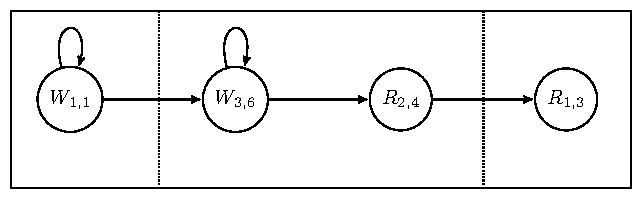
\includegraphics[width=.8\textwidth]{SlidingWindow_x.pdf}
  \caption{滑动窗口示例}\label{pic:slidingWindow}
\end{figure}
对于\ref{sec:Example}给出的实例,取表\ref{tab:exeResult}中第一个运行情况进行讨论,对变量x的访问序列是$R_{1,1}-W_{1,1}-R_{3,6}-W_{3,6}-R_{2,4}-R_{1,3}$。滑动窗口如图\ref{pic:slidingWindow} 所示。
开始是线程1连续两次对变量操作$R_{1,1}-W_{1,1}$。滑动窗口首先读入线程1的读操作$R_{1}$,接着又读入了线程1的写操作$W_{1}$,因为两次访问都是同一个线程,所以滑动窗口向前滑动,只记录$W_1$。同理,窗口内又读入了$W_3$和$R_2$。当滑动窗口已满的时候,则移除最早的记录。对于图所示的滑动窗口,窗口大小是3,当读入线程2的操作$R_{2,4}$时,窗口已满,则窗口滑动,移除最早的记录$W_{1,1}$。\par
滑动窗口的容量是有限的,如果窗口过小,可能在没有判断出模式的情况下就移除了早先的记录。如果窗口过大,又会占用过多的系统资源,从而造成Falcon的运行效率低下。所以,选择合适的滑动窗口大小也是一个复杂的问题。在Falcon论文中,作者通过试验发现当窗口大小为9的时候就足以识别所有的模式\cite{park2010falcon}。\\
\textbf{实时模式识别}\par
当滑动窗口的内容更新时,如果检测到滑动窗口已满,则扫描窗口里的记录来识别数据访问模式。识别访问模式时,首先检查是否有表格\ref{tab:UnSeInterleavingPatterns}中所列的模式。如果没有,再检查是否有表格\ref{tab:ConflictingInterleavingPatterns}中所列的模式。因此,Falcon如果已经识别到了原子性破坏的访问模式,就不会重复识别顺序破坏的模式。\par
\subsubsection{模式的可疑度排序}\label{sec:rankPattern}
Falcon的第二步是通过统计分析得到每个模式的可疑度。执行第二步时,需要第一步得到的数据访问模式和被测程序的运行结果。\par
在Falcon中,作者使用了Jaccard系数来衡量一个模式的可疑度。Jaccard系数,也被操作Jaccard相似系数,在统计学中用来被衡量两个样本集的相似性。对于集合A和B,Jaccard相似系数为:
\begin{equation}\label{ori_Jaccard}
  J(A,B)=\frac{|A\bigcap B|}{|A\bigcup B|}
\end{equation}
在Falcon工具中,可以通过衡量一个数据访问模式的通过测试集和失效测试集之间的相似性作为该模式的可疑度。对于一个模式$p$,有通过的执行数$pass(p)$,失效的执行数$failed(p)$和该被测程序所有测试失效的个数$totalfalied$,将公式\ref{ori_Jaccard}展开可以得到$p$ 的可疑度:
\begin{equation}\label{Jaccard}
    suspiciousness(p)=\frac{failed(p)}{totalfailed + passed(p)}
\end{equation}\par
对于\ref{sec:Example}中表格\ref{tab:exeResult} 给出的实例和四个数据访问模式,假设程序运行4次后的运行结果和每次运行出现的数据访问模式如表格\ref{tab:Exampleresult}所示。
\begin{table}[!ht]
  \centering
  \zihao{4}
  \caption{示例伪代码的假设运行结果}\label{tab:Exampleresult}
  \begin{tabular}{|c|c|c|c|c|c|}
     \hline
     简化的访问模式            & 运行1        & 运行2        & 运行3 & 运行4 & 可疑度 \\\hline
     x的访问模式:$W_1-W_3-R_1$ & $\checkmark$ & $\checkmark$ &       &       & 0 \\\hline
     x的访问模式:$W_1-W_2-R_1$ &              &              & $\checkmark$   & $\checkmark$   & 0.5 \\\hline
     y的访问模式:$W_1-W_3-R_1$ & $\checkmark$ &              & $\checkmark$   &       & 0 \\\hline
     y的访问模式:$W_1-W_2-R_1$ &              & $\checkmark$ &       & $\checkmark$   & 0.5 \\\hline
     运行结果                  & Pass         & Pass         & Pass  & Failed&  \\
     \hline
   \end{tabular}
\end{table}
对于第一个模式,根据公式\ref{Jaccard},可以得到它的可疑度是
\[
  suspiciousness(p)=\frac{failed(p)}{totalfailed + passed(p)}=\frac{0}{1+2}=0
\]
对于第二个模式,根据公式\ref{Jaccard},可以得到它的可疑度是
\[
  suspiciousness(p)=\frac{failed(p)}{totalfailed + passed(p)}=\frac{1}{1+1}=0.5
\]
同理,可以依次计算得到表格\ref{tab:Exampleresult}中最后一列所示的可疑度。
\subsection{本课题的目标}
本文将对指导老师所提供的Falcon源码(部分实现的版本)进行分析、补充和重构,总结错误定位工具的实现技术。进而实现Falcon工具的可视化,从而可以更加直观地展现出程序中的错误位置。\par
在本篇论文的第2章将介绍Falcon的原理和算法实现,第3章将简要介绍可视化的实现,第4章总结本次毕业设计。
